% +------------------------------------------------------------------------+
% | CGAL User Manual:  main.tex
% +------------------------------------------------------------------------+
% | R-tree User Manual
% |
% | 31.03.2000   Gabriele Neyer
% |              Start writing the user manual
% | 
\RCSdef{\hdsRev}{$Revision$}
\RCSdefDate{\hdsDate}{$Date$}
% +------------------------------------------------------------------------+
%   257  11:49   latex wrapper
%   258  11:50   makeindex wrapper
%   259  11:50   index_fix wrapper.ind
%   260  11:50   ls /pub/blabla/CGAL/Tools/3.5/scripts/index_fix wrapper.ind
%   261  11:50   latex wrapper
%   262  11:50   xdvi wrapper.dvi
% setenv TEXINPUTS .:/home/neyer/tex:/pub/blabla/tex:
% setenv LATEX_CONV_CONFIG /pub/blabla/CGAL/Tools/latex_converter_config
% setenv LATEX_CONV_HEADER /pub/blabla/CGAL/CGAL/include
% setenv LATEX_CONV_BIN /pub/blabla/sun4OS5/bin


\chapter{External Memory Data Structures} \label{Trees}

\section{R-Tree and R$^\star $-Tree}
\subsection{What we provide}
CGAL provides the  R-Tree and the R$^\star$-Tree data structures 
as dynamic index structure for spatial
searching. The design goal was to create an algorithm component
that is easily, safely, and efficiently adaptable to all common
R-trees and R$^\star$-Trees  to be used in
new unforseen contexts.

We designed the tree to be independent of the spatial objects the
tree manages, the underlying database, and to some extend
independent of the structure of the index structure. We provide
some databases and the most common components that define the
index structure of an R-tree. Note, often we simply write R-Tree
instead of R-Tree and R$^\star$-Tree.

\subsection{What is an R-tree?}
The R-Tree \cite{gutt-84} is a hierarchical data structure  that
can be viewed as a multidimensional generalization of a
B$^+$-Tree \cite{come-79}. 
It supports exact search, window queries, insertion, and deletion
of spatial objects in any dimension $d$. Usually, the smallest
$d$-dimensional aligned rectangle that encloses the spatial object (the {\em orthogonal bounding box}) is
associated with the object. The index of the tree is build
according to these orthogonal bounding boxes, which are therefore
called \ccc{ Key}s. 
Each node in the tree corresponds to the smallest $d$-dimensional
aligned rectangle that encloses its child nodes. The leaf nodes store the
actual geometric objects. The data structure of a \ccc{Key} is
not restricted to have the form of a $d$-dimensional bounding
box. One can also define another data strucure as the \ccc{Key}
data structure, e.g. the smallest enclosing circle.
%Each 
%$d$-dimensional aligned rectangle may be a container (bounding
%box) for a
%{\em geometric object} with a more complex shape. 
 
 
R-Trees are balanced in the sense that all leaf nodes appear on
the same level. 
Often, each node of the tree represents a disk block and therefore has a fixed maximum
storage capacity. Therefore, the R-Tree has variable parameters
that define the minimum and maximum size of a node or of a leaf
of the tree. \ccc{IO_max_cap_nodes} is the
maximum number of \ccc{Keys} a node can hold; \ccc{IO_min_cap_nodes}$\le\frac{\ccc{IO_max_cap_nodes}}{2}$ is the minimum number of
\ccc{Keys} a node should hold.
Just as in $B$-trees, $R$-trees guarantee for each
node except the root to have between \ccc{IO_min_cap_nodes} and \ccc{IO_max_cap_nodes}
entries; the root has between $2$ and \ccc{IO_max_cap_nodes} entries.
Since the data elements are allowed to have different sizes, we
can not define the maximum size of a leaf in terms of the number
of \ccc{Data} elements. We therefore have a parameter
\ccc{IO_page_size} which defines the maximum size of a
leaf. \ccc{IO_min_cap_leaves} defines the minmum number of
\ccc{Data} elements in a leaf.
We say that
underflow occurs if a node uses less then \ccc{IO_min_cap_nodes}
(\ccc{IO_min_cap_leaves}, resp.) entries.
Overflow occurs when we try to insert the $\ccc{IO_max_cap_nodes}+1^{st}$
entry into a node or a Data element in a leaf which exceeds the 
leaf capacity \ccc{IO_page_size}. 
%If an underflow occurs, nodes are merged or reinserted;
%if overflow occurs, the node has to be
%split. Many merging and splitting strategies  have been
%proposed. Some important ones are those from
%Guttman~\cite{gutt-84} and from Beckmann et al.~\cite{Beckmann:1990:RER}.

Note that the R-tree is not unique. Its structure depends heavily
on the order in which the individual bounding boxes were inserted
into (and possibly deleted from) the tree.
 
A new object is inserted into a leaf node. The appropriate leaf
node  is determined by traversing the R-tree starting at its root
and at each step {\bf choosing the subtree} whose corresponding
\ccc{Key} causes the minimum {\em costs} when enlarging it with
the \ccc{Key} of the new object. Various objective functions have
been proposed for the calculation of the minimum cost. The most
common functions are: the minimum area enlargement, the minimum margin
enlargement and the minimum overlap enlargement between the \ccc{Key}s of the
subtrees. 
Once the leaf node is determined, a check is made to see if the
insertion of the \ccc{Key} will cause the node to overflow. If
yes, then the node must be split, and the node entries are
distributed into two nodes. Splits are propargated
up the tree. 

Many {\bf split strategies} have been proposed. Some important ones are those from
Guttman~\cite{gutt-84} and from Beckmann et
al.~\cite{Beckmann:1990:RER}.
The goals of these strategies are to  
 partition the data entries in two
nodes such that the overlap  of these nodes is minimized, the
area is minimized, the margin is minimized or that a combination of
these criteria is optimized.  

{\bf Deletion} of an object from an R-tree proceeds by locating the
leaf node that contains the object and removing the object from the node. Then, the
covering \ccc{Key}s on the path from the root to the leaf node
are adjusted. Underflow occurs if a
node uses less than $\ccc{IO_min_cap_nodes}$
(\ccc{IO_min_cap_leaves}, resp.) entries. In this case the
underfilled node is either removed from the tree and the children
are reinserted or the elements of the underfilled node are merged
(in respect to the cost function) 
into its siblings which are the other nodes in the same level of the
tree as the underfilled node is. 

{\bf Searching} all objects that have the same \ccc{Key} as the
query \ccc{Key}, have
non empty intersection with the query \ccc{Key}, or enclose the
query \ccc{Key}, is straight forward. The only problem is that
a large number of nodes may have to be returned since a \ccc{Key}
may be contained in the covering \ccc{Key} of many nodes while
its corresponding object is contained only in one of the leaf
nodes.
Furthermore, the output of queries has to be performed
output sensitive. That is, the objects
are returned one by one in order not to exceed the
main memory capacity.

\subsection{Data Structure Design}

\begin{ccTexOnly}
\begin{figure}
%\psfrag{A}{\footnotesize\ccc{Data}}
%\psfrag{B}{\footnotesize\ccc{Key}}
%\psfrag{C}{\footnotesize\ccc{R_tree_traits}}
%\psfrag{D}{\footnotesize\ccc{R_tree}}
%\psfrag{E}{\footnotesize\ccc{IO_tree_traits}}
%\psfrag{F}{\footnotesize\ccc{IO_tree_traits}}
%\psfrag{G}{\footnotesize\hspace*{-.1cm}\parbox{1.9cm}{Database of tree nodes}}
%\psfrag{H}{\footnotesize\hspace*{-.1cm}\parbox{1.9cm}{Database of leaf nodes}}
%\psfrag{I}{\footnotesize\ccc{choose_subtree}}
%\psfrag{J}{\footnotesize\ccc{split_node}}
%\psfrag{K}{\footnotesize\ccc{split_leaf}}
%\psfrag{L}{\footnotesize\ccc{reinsertion_node}}
%\psfrag{M}{\footnotesize\ccc{reinsertion_leaf}}
%\psfrag{O}{\footnotesize\ccc{R_tree_index}}
%\psfrag{P}{\footnotesize\ccc{R_tree_storage}}
\begin{center}
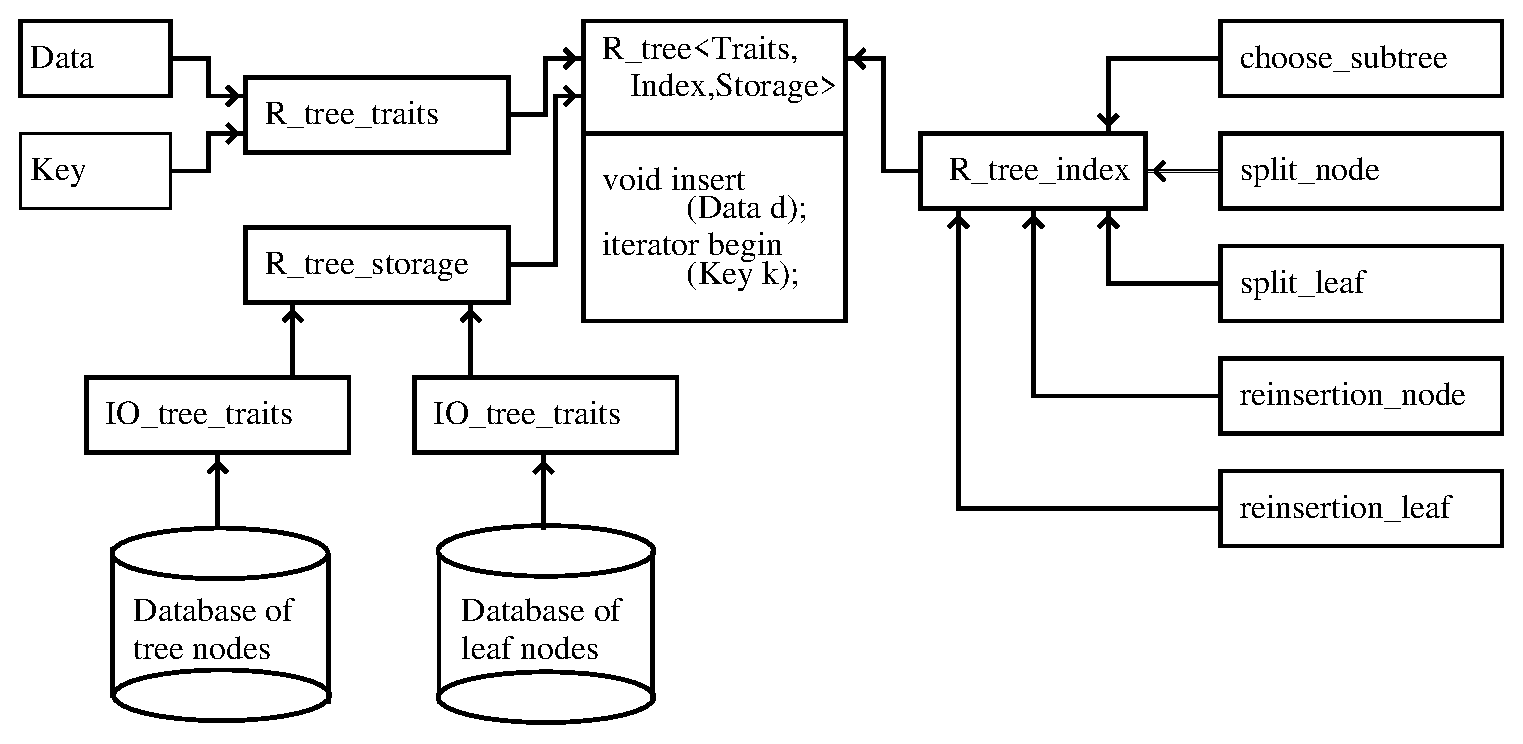
\includegraphics[width=14cm,clip]{rtree-classes4.eps}
\end{center}
\caption{\label{User:r-tree-design} R-Tree components}
\end{figure}
\end{ccTexOnly}
\begin{ccHtmlOnly}
    <!2><TABLE BORDER=0 CELLSPACING=2 CELLPADDING=0 WIDTH=650>
        <TR><TD ALIGN=LEFT VALIGN=TOP WIDTH=100% NOWRAP COLSPAN=2>
    <img border=0 src="./rtree-classes4.gif" alt="R-Tree components">
    </TD>
    <TD ALIGN=LEFT VALIGN=TOP WIDTH=50%><img border=0 src="./rtree-classes4.gif"
alt="R-Tree components">
      </TD></TR></TABLE>
\end{ccHtmlOnly}

\begin{ccTexOnly}
Figure~\ref{User:r-tree-design} shows the different components of the
R-Tree (R$^\star $-Tree) that can be plugged into the tree. 
\end{ccTexOnly}
\begin{ccHtmlOnly}
The figure above shows the different components of the
R-Tree (R*-Tree) that can be plugged into the tree. 
\end{ccHtmlOnly}
The R-Tree has three template arguments:
\begin{description}
\item[\ccc{R-tree_traits}] is the traits class which defines the
  access on the \ccc{Data} and their \ccc{Key}s. E.g. as
  \ccc{Data} you could define a 2-dimensional polygon and as
  \ccc{Key} you could define a bounding box of a
  2-dimensional polygon.
\item[\ccc{R_tree_index}] defines the indexing strategies of the
  tree. E.g. a strategy that defines in which subtree a new item
  is inserted, or how to
  split an overfull node. \cgal\/ provides predefined index
  functions for the most commonly used strategies.
\item[\ccc{R_tree_storage}] defines the databases for the inner
  nodes of the tree and the leave nodes in which the \ccc{Data}
  items are stored. The functionality of the databases is
  accessed through the traits class \ccc{IO_tree_traits}. \cgal\/
  provides a database in external memory whith variable cash size
  and a database in internal memory.
\end{description}
Instead of using the predefined classes you can always 
design your own classes. For this, please refer the reference manual.


\section{Example program}
\label{User:r-star-tree-example}
The following piece of code defines an R$^\star$-Tree.
The \ccc{Data} type simply defines an \ccc{R_tree_key_2} type as
\ccc{Key} data type. The \ccc{R_tree_traits} class implementation
is instanciated with this \ccc{Data} type.
As \ccc{R_tree_index} class we chose the predefined
\ccc{R_star_tree_index} class. As \ccc{R_tree_storage} class we
chose the \ccc{R_tree_external_storage} class.

An R$^\star$-Tree is created and 16 2-dimensional squares are
inserted. Then, it is iterated through all elements of the tree
and various queries are performed. Furthermore, some elements are
deleted.



\ccExample
\begin{cprog}
#include <CGAL/R_tree.h>
#include <CGAL/R_tree_key.h>
#include <CGAL/R_star_tree_index.h>
#include <CGAL/R_tree_traits_example.h>
#include <CGAL/R_tree_external_storage.h>
#define NUMBER 16

/* Definition of the data type */
struct Data{
public:
  typedef CGAL::R_tree_key_2 Key;
  Key key;
  size_t size(void) const {
    return sizeof(*this);
  }
  void read(char ** s) {
    key.read(s);
  }
  void write(char * s) {
    key.write(s);
  }    
  void dump(int level =0){
    key.dump();
  }
};

/* definition of the R_tree_traits - depending on the Data type */
typedef CGAL::R_tree_traits<Data> TTraits; 
typedef Data::Key Key;

/* definition of the R_Tree that contains Data elements, uses 
   Star Tree index structure and stores the elements in 
   external memory */
typedef CGAL::R_tree<TTraits, CGAL::R_star_tree_index<TTraits>,
  CGAL::R_tree_external_storage> R_Tree_Inst;

int main() {
  TTraits traits;
  Data  elem; 
  int k; 
  Key key= Key(0,2,0,2);
  std::vector<Data > source;
  /* creation of R_tree associated to the files: */
  R_Tree_Inst r_star_tree("__star_tree.head","__star_tree.dat", 
                          "__star_leaf_data.dat");

  /* create 2-dimensional squares as input data */
  for (k=0;k<NUMBER;++k) {
    elem.key=key;
    source.push_back(elem);
    key.xmin++; key.ymin++; key.xmax++; key.ymax++;
  }

  /* Insertion of the data elements */
  for (k=0;k<NUMBER;++k) {
    r_star_tree.insert(source[k]);
  }
  r_star_tree.dump();

  std::cerr<< "Iteration through all elements of the tree\n";
  R_Tree_Inst::iterator it_begin=r_star_tree.begin();
  R_Tree_Inst::iterator it_end=r_star_tree.end();
  while(it_begin != it_end){
    std::cerr << "------------";
    (*it_begin).dump();
    ++it_begin;
  }
  std::cerr<< "End of iteration through all elements of the tree\n";

  std::cerr<< "Iteration through all elements of the tree\n";
  std::cerr<< "that have non empty intersection with source[0].key=(0,2,0,2)\n";
  it_begin=r_star_tree.begin(source[0].key);
  it_end=r_star_tree.end(source[0].key);
  while(it_begin != it_end){
    std::cerr << std::endl;
    (*it_begin).dump();
    ++it_begin;
  }
  std::cerr<< "End of iteration through the query elements of the tree\n";

  std::cerr<< "Iteration through all elements of the tree\n";
  std::cerr<< "that enclose source[2].key=(2,4,2,4)\n";
  it_begin=r_star_tree.begin_enclose(source[2].key);
  it_end=r_star_tree.end_enclose(source[2].key);
  while(it_begin != it_end){
    std::cerr << std::endl;
    (*it_begin).dump();
    ++it_begin;
  }
  std::cerr<< "End of iteration through the query elements of the tree\n";

  std::cerr<< "Iteration through all elements of the tree\n";
  std::cerr<< "that compare source[4].key=(4,8,4,8)\n";
  it_begin=r_star_tree.begin_compare(source[4].key);
  it_end=r_star_tree.end_compare(source[4].key);
  while(it_begin != it_end){
    std::cerr << std::endl;
    (*it_begin).dump();
    ++it_begin;
  }
  std::cerr<< "End of iteration through the query elements of the tree\n";

  std::cerr << "Check for elements that intersects source[1].key=(1,2,1,2)\n";
  if(!r_star_tree.find_key_intersect(source[1].key))
    {
      std::cerr << "no key intersection of "; 
      traits.dump(traits.build(source[1]));
    }
  else
    std::cerr << "key intersection = true";

  std::cerr << "Check for elements that intersects source[1].key=(1,2,1,2)\n";
  if(!r_star_tree.find_key_include(source[1].key))
    {
      std::cerr << "no key include of"; 
      traits.dump(traits.build(source[1]));
    }
  else
    std::cerr << "key include = true";

  Data data_del;
  std::cerr << "Deletion of all data with key source[0].key=(0,2,0,2)\n";
  while(r_star_tree.delete_key(source[0].key,data_del))
    traits.dump(data_del.key);
  std::cerr << "Deletion of all data with key source[1].key=(1,3,1,3)\n";
  while(r_star_tree.delete_key(source[1].key,data_del))
    traits.dump(data_del.key);
  std::cerr << "Deletion of all data with key source[2].key=(2,4,2,4)\n";
  while(r_star_tree.delete_key(source[2].key,data_del))
    traits.dump(data_del.key);

  std::cerr << "Check for elements that intersect source[1].key=(1,2,1,2)\n";
  if(!r_star_tree.find_key_intersect(source[1].key))
    {
      std::cerr << "no key intersect of"; 
      traits.dump(traits.build(source[1]));
    }
  else
    std::cerr << "key intersect = true";
}
\end{cprog}

Class \ccc{R_tree_key_2} looks like this:

\begin{cprog}

/* R_tree_key_2 is a 2 dimensional rectangle. */
class R_tree_key_2
{
  int min(int a, int b) const { return (a<b) ? a : b; }
  int max(int a, int b) const { return (a<b) ? b : a; }
public:
  int xmin, xmax, ymin, ymax;
  size_t size(void) const {
    return 4*sizeof(int)+4;
  }

  R_tree_key_2(){xmin=xmax=ymin=ymax=0;}
  R_tree_key_2(int x1, int x2, int y1, int y2){
    xmin=x1; xmax=x2; ymin=y1; ymax=y2;
  }
  
  R_tree_key_2(const R_tree_key_2 &t){
    xmin=t.xmin; xmax=t.xmax; ymin=t.ymin; ymax=t.ymax;
  }
      
  bool operator==(const R_tree_key_2 &p) const {
    return ((xmin==p.xmin) && (xmax == p.xmax) 
            && (ymin == p.ymin) &&(ymax == p.ymax));
  }

  R_tree_key_2 & operator=(const R_tree_key_2 &t)  {
    xmin=t.xmin; xmax=t.xmax; ymin=t.ymin; ymax=t.ymax;
    return *this;
  }

  class C_Compare_1{
  public:
    bool operator()(const R_tree_key_2 &p, const R_tree_key_2 &q)
    {
      if(p.xmin < q.xmin)
        return true;
      else 
        if(p.xmin==q.xmin)
          if(p.xmax < q.xmax)
            return true;
      return false;
    }
  };

  class C_Compare_2{
  public:
    bool operator()(const R_tree_key_2 &p, const R_tree_key_2 &q)
    {
      if(p.ymin < q.ymin)
        return true;
      else 
        if(p.ymin==q.ymin)
          if(p.ymax < q.ymax)
            return true;
      return false;
    }
  };
  typedef C_Compare_1 compare_1;
  typedef C_Compare_2 compare_2;

  void unify( const R_tree_key_2 & p, const R_tree_key_2 & q){
    xmin = min(p.xmin, q.xmin); xmax = max(p.xmax, q.xmax);
    ymin = min(p.ymin, q.ymin); ymax = max(p.ymax, q.ymax);
  }

  /* returns true if *this includes y */
  bool include(const R_tree_key_2& y) const {
    if ((xmin > y.xmin) || (ymin >  y.ymin))
      return false;
    if ((xmax < y.xmax) || (ymax < y.ymax))
      return false;
    return true;
  }
  
  bool compare(const R_tree_key_2 & y) const{
    return intersect(y);
  }

  bool intersect( const R_tree_key_2& y) const {
    if ((xmax <= y.xmin) || (y.xmax <= xmin)) {
      return false;
    }
    if ((ymax <= y.ymin) || (y.ymax <= ymin)) {
      return false;
    }
    return true;
  } 

  double cost() const {
    return (xmax - xmin) * (ymax - ymin);
  }

  void intersection( const R_tree_key_2 & p, const R_tree_key_2 & q){
    if(p.intersect(q))
      {
        xmin = max(p.xmin, q.xmin); xmax = min(p.xmax, q.xmax);
        ymin = max(p.ymin, q.ymin); ymax = min(p.ymax, q.ymax);
      }
  }

  /* compute the distance between the centers of the keys */
  double center_dist( const R_tree_key_2& q) const {
    double x=xmin + 0.5*(xmax-xmin);
    double y=ymin + 0.5*(ymax-ymin);
    double qx=q.xmin + 0.5*(q.xmax-q.xmin);
    double qy=q.ymin + 0.5*(q.ymax-q.ymin);
    double dist = (x-qx)*(x-qx) + (y-qy)*(y-qy); 
    return dist;
  }

  void read(char **s) {
    int sint=(int)sizeof(int);
    char *from_int=new char[sint];
    
    int i,r=0;
    for (i=0; i<sint; i++)
      from_int[i] = (*s)[i];
    r += sint;
    xmin=*((int *)from_int);

    for (i=0; i<sint; i++)
      from_int[i] = (*s)[i+r];
    r += sint;
    xmax=*((int *)from_int);

    for (i=0; i<sint; i++)
      from_int[i] = (*s)[i+r];
    r += sint;
    ymin=*((int *)from_int);

    for (i=0; i<sint; i++)
      from_int[i] = (*s)[i+r];
    r += sint;
    ymax=*((int *)from_int);

    delete[] from_int;
  }

  void write(char **s)
    {
      int sint=(int)sizeof(int);
      char *from_int=new char[sint];
      int i,r=0;
      memcpy(from_int,(char *)(&xmin),sint);
      for (i=0; i<sint; i++)
        (*s)[i] = from_int[i];
      r += sint;

      memcpy(from_int,(char *)(&xmax),sint);
      for (i=0; i<sint; i++)
        (*s)[i+r] = from_int[i];
      r += sint;

      memcpy(from_int, (char *)(&ymin),sint);
      for (i=0; i<sint; i++)
        (*s)[i+r] = from_int[i];
      r += sint;

      memcpy(from_int, (char *)(&ymax),sint);
      for (i=0; i<sint; i++)
        (*s)[i+r] = from_int[i];

      delete[] from_int;
    }

  void dump(int depth=0) const  {
    std::cerr << "(" << xmin << "/" << ymin 
         << "),(" << xmax << "/" << ymax << ")";
  }

};

std::ostream& operator << (std::ostream& s, R_tree_key_2 m) {
  s  << "(" << m.xmin << "/" << m.ymin << ")("
     << m.xmax << "/" << m.ymax << ")" << std::endl;
  return s;
}
\end{cprog}

\newpage

% As long as there is only one manual we include this here:
\input{reference.tex}
